\section{Uppgift 5}\label{uppgift-5}

\subsection{Instruktioner}
\begin{verbatim}
5. Skriv ett program där användaren ska skriva in ett heltal. Programmet ska
   sedan skriva ut alla heltal från detta tal ner till ett. Du ska använda dig
   av en while-loop. Exempel på utskrift, användarens inmatning är markerat med
   fetstil/understrykning:

    Ange det heltal som du vill räkna ner från: *6*
    6 5 4 3 2 1
\end{verbatim}

\subsection{Lösning}
\subsubsection{Funktion}
En \texttt{static final} variabel \texttt{QUERY} håller en textsträng som ska
skrivas ut till användaren senare under programmets exekvering.
Variabler med enbart versaler är en slags globala variabler som kan modifieras
av programmeraren, likt det en gör med \texttt{\#define} i C-liknande språk för
att undvika att ''hårdkoda'' t.ex. textsträngar.
\par Logiken för att kontrollera korrekt inmatning är samma som den i Uppgift
\ref{uppgift-4}.
\par När variabeln \texttt{start} innehåller ett positivt heltal används en
\texttt{while}-loop för att skriva ut en nedräkning på skärmen. Extra mellanslag
läggs till genom att textsträngen \texttt{start} och ett mellanslag 
\texttt{(''\ '')} konkateneras genom summering, en funktion som särskiljer Java.

\subsubsection{Källkod}\label{uppgift-5_src}
\subsubsection*{Lab1Uppg05.java}
%\begin{listing}[H]
    \inputminted[linenos]{java}{src/Lab1Uppg05.java}
    \caption{Lab1Uppg05.java}
    \label{Uppg5src}
%\end{listing}

\subsubsection{Skärmdump}
\begin{figure}[htbp]
    \centering
        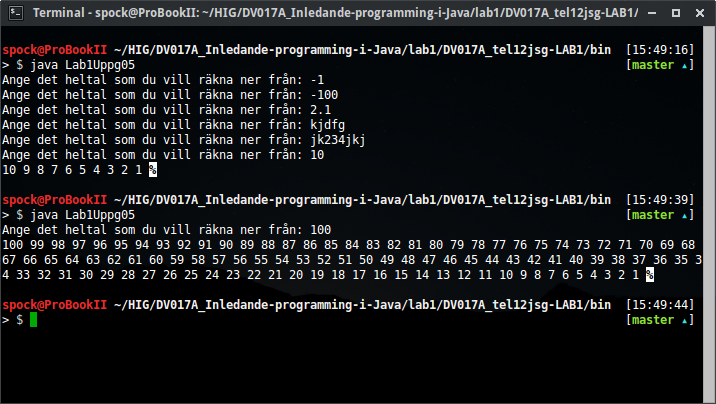
\includegraphics[width=\linewidth]{img/05.png}
    \caption{Körning av koden till Uppgift \ref{uppgift-5}}
    \label{fig:screenshot-05}
\end{figure}
